\title{\Large Projet d'ingénierie\\
        \emph{Intelligent Digital Systems} \\
        \bf\Large iGlove \\
        Contrôle d’objets connectés au doigt}
\author{\large Florent Pollet \ \\}
\date{\large\today}

\makeatletter
    \begin{titlepage}
        \begin{center}
	   { 
\includegraphics[width=8cm]{imgs/mp_logo.png}}
	   {\ \\ \ \\}
        \vbox{}\vspace{1cm}
            {\@title }\\[0.5cm] 
            %{ \includegraphics[width=7cm]{imgs/cover.PNG}}\\[1cm]

            {
                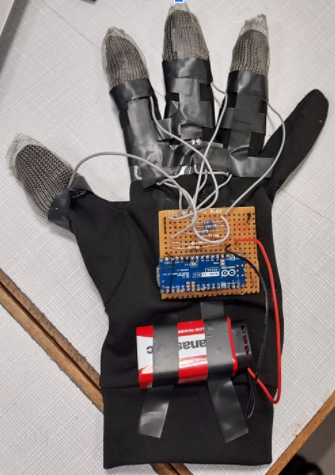
\includegraphics[width=0.3\textwidth]{imgs/Gant.png}
            }

            {\large \ \\ Equipe: Thibaut Cailleriez, Jean-Edouard Dupau, Pierre Marié, Alondra Alfaro et \bf Florent Pollet\ \\}
            {\large \ \\ Encadrants: \bf Cyril Joly et Bodgan Stanciulescu\ \\}
            \vspace{1cm}
            {\@date\\}
            \vspace{0.5cm}

        \end{center}



        \begin{remerciements}
            Je tiens à remercier les encadrants Cyril Joly et Bogdan Stanciulescu pour 
             l'organisation des conférences avec des intervenants de centres de recherche et d'entreprises,
             leurs cours passionnants d'électronique embarquée
             et leur aide ainsi que leur encadrement tout au long du projet.
            Je souhaite également remercier David Mazouz pour son soutien et ses conseils pratiques.
            Cela a été une expérience très formatrice et intéressante de travailler en équipe à la réalisation d'un prototype
             fonctionnel en un temps restreint.
        \end{remerciements}
    
    

    \end{titlepage}


    \makeatother